%%%%%%%%%%%%%%%%%%%%%%%%%%%%%%%%%%%%%%%%%
% Stylish Article
% LaTeX Template
% Version 2.1 (1/10/15)
%
% This template has been downloaded from:
% http://www.LaTeXTemplates.com
%
% Original author:
% Mathias Legrand (legrand.mathias@gmail.com) 
% With extensive modifications by:
% Vel (vel@latextemplates.com)
%
% License:
% CC BY-NC-SA 3.0 (http://creativecommons.org/licenses/by-nc-sa/3.0/)
%
%%%%%%%%%%%%%%%%%%%%%%%%%%%%%%%%%%%%%%%%%

%----------------------------------------------------------------------------------------
%	PACKAGES AND OTHER DOCUMENT CONFIGURATIONS
%----------------------------------------------------------------------------------------

\documentclass[fleqn,10pt]{SelfArx} % Document font size and equations flushed left

\usepackage[english]{babel} % Specify a different language here - english by default

\usepackage{lipsum} % Required to insert dummy text. To be removed otherwise
\usepackage{float}
\usepackage{blindtext}
\usepackage{listings}
\usepackage[utf8]{inputenc}
\usepackage{color}
\usepackage{framed}
%----------------------------------------------------------------------------------------
%	COLUMNS
%----------------------------------------------------------------------------------------

\setlength{\columnsep}{0.55cm} % Distance between the two columns of text
\setlength{\fboxrule}{0.75pt} % Width of the border around the abstract

%----------------------------------------------------------------------------------------
%	COLORS
%----------------------------------------------------------------------------------------

\definecolor{color1}{RGB}{0,0,90} % Color of the article title and sections
\definecolor{color2}{RGB}{0,20,20} % Color of the boxes behind the abstract and headings

%----------------------------------------------------------------------------------------
%	HYPERLINKS
%----------------------------------------------------------------------------------------

\usepackage{hyperref} % Required for hyperlinks
\hypersetup{hidelinks,colorlinks,breaklinks=true,urlcolor=color2,citecolor=color1,linkcolor=color1,bookmarksopen=false,pdftitle={Title},pdfauthor={Author}}

%----------------------------------------------------------------------------------------
%	ARTICLE INFORMATION
%----------------------------------------------------------------------------------------

\JournalInfo{Data Mining B565 Fall 2016} % Journal information
\Archive{} % Additional notes (e.g. copyright, DOI, review/research article)

\PaperTitle{Semester Project} % Article title

\Authors{Ethan Li\textsuperscript{1}*, Saheli Saha\textsuperscript{1}} % Authors
\affiliation{\textsuperscript{1}\textit{Computer Science, School of Informatics and Computing, Indiana University, Bloomington, IN, USA}} % Author affiliation 
\affiliation{*\textbf{Corresponding author}: li526@indiana.edu} % Corresponding author

\Keywords{Data mining --- Prediction --- Regression} % Keywords - if you don't want any simply remove all the text between the curly brackets
\newcommand{\keywordname}{Keywords} % Defines the keywords heading name

%----------------------------------------------------------------------------------------
%	ABSTRACT
%----------------------------------------------------------------------------------------

\Abstract{We have participated into two Kaggle Competitions as our Data Mining semester project: House Prices and Outbrain Click Prediction. After a lot of well-designed experiments with carefully-chosen techniques and algorithms, we got our best results with Lasso Regression and Field-Aware Factorization Machines with Leakage respectively.  For House Prices Prediction problem, we found out that feature engineering is very important since improved approaches to clean the data gave us much better LB score and ranks on Kaggle. However, parameter tuning on almost all algorithms gave similar kind of scores while applied on the same cleaned data. In Outbrain click prediction, sampling and streaming are successfully used to handle this big dataset. By sampling we are able to use only ten percents of training data to get similar outputs as using the whole data. Very powerful yet rarely found concept Data leakage improved Outbrain Click prediction a lot. Finally for both the project we concluded that feature engineering is more important than parameter tuning. Using these approaches we got 0.12188 for House Price prediction and  0.64077 in Outbrain Click Prediction.}

%----------------------------------------------------------------------------------------

\begin{document}

\flushbottom % Makes all text pages the same height

\maketitle % Print the title and abstract box

All the work herein is solely ours.

Group name: Mesa

\tableofcontents % Print the contents section

\thispagestyle{empty} % Removes page numbering from the first page

%----------------------------------------------------------------------------------------
%	ARTICLE CONTENTS
%----------------------------------------------------------------------------------------

\section*{Introduction} % The \section*{} command stops section numbering

\addcontentsline{toc}{section}{Introduction} % Adds this section to the table of contents
  
We are living in the big data age. Peta-bytes of data are produced every day in the world. The traditional data analysis techniques no longer satisfy the need of uncovering valuable information from such huge amount of data, which led to the birth of data mining.

Data mining is the process of discovering interesting patterns and knowledge from large amount of data \cite{han2011data}. Data mining tasks can be divided into two major categories \cite{pang2006introduction}: i) predictive tasks. The objective of these tasks is to predict the value of a particular attribute based on the values of other attributes. It includes classification and regression tasks. ii) Descriptive tasks. The objective is to derive patterns (correlations, trends, clusters, trajectories and anomalies) that summarize the underlying relationships in data.

In this report, we discuss about regression problems by showing two specific examples from Kaggle.com,  which are house prices prediction\cite{kaggle:house}  and Outbrain click prediction\cite{kaggle:outbrain}  problems. The description of these two problems are as follows.
  
\subsection{House Prices Prediction}
The House Prices problem is a general regression problem. With 79 explanatory variables describing (almost) every aspect of a residential home, for example, the building class, the type of utilities available and the style of dwelling etc,  in Ames, Iowa. This competition challenges us to predict the final price of each home. We are provided with the training set, test set,  data description and the sample submission which is a benchmark submission from a linear regression on year and month of sale, lot square footage and number of bedrooms are provided. Our goal on this problem is to investigate and propose our solutions to get better prediction accuracy.

\subsection{Outbrain Click Prediction}
Outbrain Click Prediction is a Click-through Rate Prediction (CTR) problem. CTR of an advertisement is the number of clicks on an advertisement divided by the number of times the advertisement is shown (impressions) \cite{wiki:CTR}. CTR is important because it's a measurement of the success of an online advertising campaign. High CTR of an advertisement reflects the effectiveness of the investment, which is one of the major concerns of the advertisers. One way to improve CTR is to estimate the possible CTR, from which the advertisers can adjust their strategy on advertising.
\begin{equation}
CTR = \frac{number\ of\ clicks}{impressions} \times 100\%
\end{equation}

On the Outbrain Click Prediction problem on Kaggle.com, we are challenged to predict which pieces of content its global base of users are likely to click on. The dataset for this challenge contains a sample of users' page views and clicks, as observed on multiple publisher sites in the United States between 14-June-2016 and 28-June-2016. Each viewed page or clicked recommendation is further accompanied by some semantic attributes of those documents. The dataset contains numerous sets of content recommendations served to a specific user in a specific context. Each context (i.e. a set of recommendations) is given a display\_id. In each such set, the user has clicked on at least one recommendation. The identities of the clicked recommendations in the test set are not revealed. The task is to rank the recommendations in each group by decreasing predicted likelihood of being clicked. This is a very large relational dataset. The page views log (page\_views.csv) is over 2 billion rows and 100GB uncompressed. 

The remaining part of this report is structured as follows. Section~\ref{background} provides background information on the data mining algorithms we are using in this report. Section~\ref{methodology} provides the details of the proposed method for these two projects. Section~\ref{experiments} describes our experimental validation methodology and results, and finally, Section~\ref{conclusion} concludes the report.
%------------------------------------------------

\section{Background}\label{background}

\subsection{Lasso Regression}
Lasso Regression \cite{tibshirani1996regression} is a popular regression algorithm. Suppose that we have data $(X^i,y)$, where i = 1,2,....,N and $x^1 = (x_i1,....., x_ip)^T$ are the predictor variables and $y_i$ are the responses. As in the regression set up we assume either the observations are independent or the $y_i s$ are conditionally independent, given the $x_ij s$. We assume that the $x_ij$ are standardized, so that $\sum_i x_ij/N = 0$, $\sum_i x_{ij}^{2}/N = 1$.

Letting $\hat{\beta}$ = $(\hat{\beta}_1,...., \hat{\beta}_p )^T$, the Lasso estimate $(\hat{\alpha}, \hat{\beta})$ is defined by,
\begin{equation}\label{lasso}
    \begin{split}
(\hat{\alpha}, \hat{\beta}) = arg min\{\sum_{i=1}^{N}(y_i - \alpha - \sum_j \beta_j - x_{ij} )^2\}\\
 Subject\ to \sum_j \mid \beta_j \mid \leq t.
\end{split}
\end{equation}
 
Here, $ t \geq 0$ is a tuning parameter. Now for all t, solution for $\alpha$ is $\hat{\alpha}$ = $\bar{y}$. We can assume that the loss of generality $\bar{y}$ = 0 and hence omit $\alpha$.

Solution of equation~\ref{lasso} is a quadratic programming problem with linear inequality constraint. The parameter t $\geq$ 0 controls the amount of shrinkage that is applied to the estimates.

\subsection{Field-aware Factorization Machines}
Field-aware Factorization Machines (FFMs) \cite{juan2016field} is a variant of factorization machines (FMs) \cite{rendle2010factorization}. It recently outperforms existing models in some world-wide CTR-prediction competitions. FMs is target for solving feature combination problems in sparse data situation. The formula of the model is:
\begin{equation}
y(x) = w_0 + \sum_{i=1}^{n} w_i x_i + \sum_{i=1}^{n}\sum_{j=i+1}^{n}<v_i, v_j>x_i x_j
\end{equation}
Here, $v_i$ is the latent variable of $i^{th}$ dimension, and $k$ $(k << n)$ is the length of latent vectors. 

FFMs adds the field concept to FMs. It categorized features based on their properties. For example, if the features are all about people's jobs, then these features should be in the same field. By introducing the fields, the formula of the model is changed to be:
\begin{equation}
 y(x) = w_0 + \sum_{i=1}^{n} w_i x_i + \sum_{i=1}^{n}\sum_{j=i+1}^{n}<v_{i,f_{j}}, v_{j,f_{i}}>x_i x_j
\end{equation}
Here, $f_i$ is the field which the $i^{th}$ feature belongs to.

Libffm\cite{libffm}, a library for field-aware factorization machines, is available to use for training and testing FFM model.

%------------------------------------------------

\section{Algorithm and Methodology} \label{methodology}

\subsection{House Prices Prediction}

 \subsubsection{Data Analysis}

The Ames, Iwoa dataset is the dataset on which we are doing the prediction on. 
It is comprised of seventy nine features to describe the Houses to be sold. In this Ames Dataset 
all the features are the variables that a buyer would like to know before buying any house.

There are fourteen discrete features to describe any particular house. Such as Number of Kitchens, type of bathroom i.e: Half or Full, Type of Street accessed to the property Gravel or Paved. Additionally Garage type or Land-slope types are also provided. 

There are twenty features to describe the dimension of the houses. It is  described in detail with the combination of common features like Lot Size, Dwelling Size and extraneous features like, Basement's Dimension, Living Area or Porch's dimension.Again these dimensions are divided into categorical data.

Large number of categorical data provided to analyze, Twenty Three nominal and twenty three ordinal data. These data varies in a large way. One or two features like Street, has two kinds of values- Gravel or Paved. Many attributes like Neighbourhood or Type of Exteriors varies from seventeen to twenty five different kinds of values.

We have categorized some features depending on the approaches we are using. For example the features which are describing the quality of the House, (ExterQual, BsmtQual, HeatingQC, KitchenQual, FireplaceQu, GarageQual, PoolQC, Fence) are considered as Ordinal Data, we have ranked those data in a scale of 0 to 10.  


\subsubsection{Data Cleaning}

For the house price prediction this is the main section to work on. After going through the data we realize proper approach to clean the data will give us more accurate results.  For each and every feature we have taken certain approaches to clean that. 

One of the data cleaning processes is to converting categorical variables to numerical variables. Although different algorithms are there, we preferred to analyze the nature of the features and then we started doing engineering on that.

At first we removed all NA values in a meaningful manner.
For example in Alley NA means no Alley so we replaced NA there with No Alley.
We did same with BsmtQual, BsmtCond, BsmtExpo, BsmntFintype1, BsmntFintype2, Fence and SaleCondition.

After transforming the values in order to make it numerical we ranked it in numerical scale. Features like Utilities, HeatingQC, SaleCondition are ranked with 0 and 1 as they have only two kind of values.

Features like ExterQual, ExterCond or KitchenQual which has five different kind of values has ranked those from one to five. Features which has NA in their value and transformed to zero are ranked from zero to five such as BsmtCond, FireplaceQu.

Features with three different kind of qualities are ranked between zero to three according to their conditions. For example OverallCond has one to nine rating. Now I have combined these values in zero to three, from low to high rating respectively.

Features like BsmtFinType1 or BsmtFinType2 which has eight different kinds of values are merged into two type of values- zero and one according to their condition.

Eventually for better result important features like LotFrontage,	LotArea, OverallQual, OverallCond, ExterQual, ExterCond, BsmtCond, GarageQual, GarageCond, KitchenQual, HeatingQC, HeatingQC, MasVnrType, SaleCondition, Reconstruct and ReconstructAfterBuy are calculated as polyvariate values after transforming the NA values to zero.

Finally we used Dummy Variable Algorithm for features like Exterior1st, Exterior2nd, RoofMatl, Condition1, Condition2 and BldgType. 

\subsubsection{Methodology}

After cleaning the data there are several algorithms that we can apply to predict the house price. We started experimenting with different regression techniques. For the cleaned data that we have organized Lasso regression proved to be the best choice. 

Regression\cite{wiki:regression} can be defined as a statistical model for prediction, which estimate relationship among variables. It includes techniques like modelling, analyzing, feature selection depending on the dependent and independent variables.

Lasso Regression is one of the regression technique which does both regression and feature selection. Hence, we have not used any other feature selection algorithm on our clean data while using Lasso Regression.

\subsubsection{Implementation}
Lasso regression have powerful statistical and computational advantages and it provides a simplicity and sparsity to the solution. 
We have used Python to clean and predicting the house sale price. 

Python has very useful packages like pandas and numpy for storing and cleaning the data respectively.

For applying the algorithm we have used Sci-kit learn package of Python\cite{wiki:scikit}. It is a free software machine learning library in python which supports classification, regression and clustering algorithms. We have used Lasso Regression as mentioned in  table~\ref{tab:lasso-code}.

Table~\ref{tab:lasso-code} described how we used Sklearn package to apply Lasso function in our Train Data first and then on the Test Data for predicting house price.

\subsection{Outbrain Click Prediction} 

\subsubsection{Data Analysis}
We are provided with eleven data files as shown in table~\ref{tab:files}. The overview of the dataset is shown in table~\ref{tab:overview}. Among all these features, what interest us the most are document topics, document category, advertiser and campaign. Since the target for this problem is to determine if each user will click on the ads or not. If one ad is clicked on, it may indicates that users are interested in the document which the ad lands on. The interests can be reflected through topics and categories. On the other hand, if an ad is clicked on, it may refer that users are interested in the products from the advertiser or the advertising campaign. If the users are interested in this product provided by specific advertiser/campaign, then they might be also interested in their other products. As for entities, the number of entities is much larger than the number of ads we are predicting on. It would not help with the prediction and might cause over-fitting. For source\_id and publisher\_id, we think they don't matter because we assume that no click behavior will be influenced by who published the documents. So in this report, we proposed our prediction methodology by using four features, which are topics, categories, advertisers and campaigns. Besides that, data "leakage" is mined in the dataset and which is very important for prediction. The discussion is in section~\ref{leak}.

\begin{table*}
\begin{framed}
\begin{lstlisting}[language=Python]
import pandas as pd
import numpy as np
from sklearn.linear_model import Lasso
model_lasso = Lasso(alpha=5e-4, max_iter=50000).fit(X_train, y)
coef = pd.Series(model_lasso.coef_, index = X_train.columns).sort_values()
imp_coef = pd.concat([coef.head(10), coef.tail(10)])
\end{lstlisting}
\end{framed}
\caption{lasso regression in python}\label{tab:lasso-code}
\end{table*}


\begin{table*}[!htbp]
\begin{center}
  \begin{tabular}{ c|c }\hline \hline
  File Name  & Description    \\ \hline \hline
  clicks\_train & indicate the ad is the display is clicked or not\\
  clicks\_test & the test data to predict \\
  events  &  information on the display\_id context\\
  promoted\_content &  details about the ads \\
  documents\_categories & the confidence that given categories was referred to in the document\\
  documents\_meta & the source\_id,publisher\_id,publish\_time of the document\\
  documents\_entities & the confidence that given entities was referred to in the document\\
  documents\_topics & the confidence that given topics was referred to in the document\\
  page\_views &  a the log of users visiting documents.  \\
  page\_views\_sample & a sample of the page\_views\\
  sample\_submission & a sample submission \\  \hline\hline
   \end{tabular}
\end{center}
\caption{Data files}\label{tab:files}
\end{table*}


\begin{table*}[!htbp]
\begin{center}
  \begin{tabular}{ ccccc }
    \hline
    feature/file          & unique IDs & min ID & max ID & Notes \\ \hline\hline
    topic\_id         &      300       &    0       &   299    &    \\
    category\_id   &      97         &   1000  &   2100  &    \\
    advertiser\_id &      4385     &   2        &   4532  &    \\
    campaign\_id &      34675   &   1        &  35554 &     \\
    entity\_id        &   1326009  &             &             &    \\
    document\_id &   2495423  &   1        & 2999333 & in doc\_topics.csv\\
    ad\_id             &    559583   &   1        & 573098   & in promoted\_content.csv\\
    ad\_id             &   478950    &   1        & 548019  & in clicks\_train.csv \\
    ad\_id            &   381385    &   1        & 567073  & in clicks\_test.csv  \\
    ad\_id            &     544300   &   1       &   567073 & in clicks\_test.csv and train\_test.csv \\
   doc\_id           &       2999334 &   1      &   2999334 & in doc\_meta.csv \\
   source\_id      &     14394     & 1         &  14404     &  NAs exist \\
   publisher\_id   &       1259     &  2       &   1263      &  NAs exist \\
    \hline\hline
  \end{tabular}
\end{center}
\caption{Overview of the datasets}\label{tab:overview}
\end{table*}

\subsubsection{Model}
It's always difficult to choose a proper model for specific data mining problems. Choosing a good model depends on problem settings and also relies on data scientist's experience. FFMs recently outperforms existing models in some world-wide CTR-prediction competitions \cite{juan2016field}. It adopts field concepts to categorize similar features to one field, for example, different jobs belong to "job" field. Here in this problem, all the features are in high dimension. For the topic feature, there are 300 unique topic\_ids; and for the campaign feature, 34k unique ids. Firstly every dimension of these categorial features will be as new features. And every original feature will be one field. The transformed data is shown in table~\ref{tab:ffm}. 

\begin{table}[!htbp]
\begin{center}
  \begin{tabular}{ c|c|c }\hline
  Field         &     Field\_ID    &     Feature\_ID\_Range \\ \hline \hline
  topic         &        0             &     [0,299] \\
  category   &        1             &     [300, 399] \\
  advertiser &        2              &    [400, 4799] \\
  campaign  &        3              &    [4800, 40353]\\ \hline \hline
  \end{tabular}
\end{center}
\caption{Data in Libffm format}\label{tab:ffm}
\end{table}

\subsubsection{Streaming and Sampling}
Faced with such large dataset, it's unfeasible to simplely join these data files by force on small memory machines. One way to enable the operation is by streaming the data to memory and performing joining operation by specific order to avoid unnecessary memory consumption. Through this we are able to join the data in our own laptop, which only has at most 4GB memory.

After transforming the data to FFM format, the size of the aggregated training data file is about 11GB, which is very huge regarding to the limited memory space of personal computer. We have to perform the experiments on-disk, which is very slow. However, we found out that using randomly sampled 10\% of the training data got the similar accuracy with the full training dataset. So in the experiments afterwards, we use sampled 10\% of training data to save memory space and reduce training time.

\subsubsection{Leakage}\label{leak}
One very important factor to solve in the click prediction problem is to apply the data leakage. Data leakage is the creation of unexpected additional information in the training data, allowing a model or machine learning algorithm to make unrealistically good predictions. Here in this problem, since the log of user visiting pages is released to us, it's possible to know that some specific users visiting some specific documents at any particular timestamp. The prediction goal is to know whether the specific user will click on specific ads or not. If we can get the information of which user visited any particular document that the ad lands on, then it is convenient to infer that the user clicked on the specific ads. The leak helps the score on pubic leaderboard on Kaggle by around 0.016.

\section{Experiments and Results}\label{experiments}
\subsection{House Prices Prediction}

\subsubsection{Experimental Setup}


As part of the data cleaning process first we have used many plotting to understand nature and the cleaning method. 
For example we have considered Sale condition as a very important feature for this prediction. The correlation of this feature is shown in Figure~\ref{fig:Figure3}.

\begin{figure}[ht]\centering % Using \begin{figure*} makes the figure take up the entire width of the page
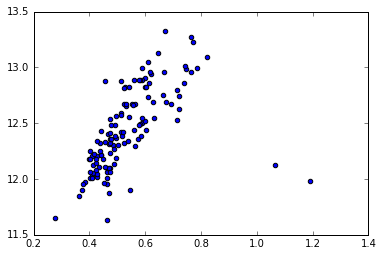
\includegraphics[width=\linewidth]{Figure3}
\caption{Nature of Sale Condition Feature}
\label{fig:Figure3}
\end{figure}

At first we applied Dummy Variable Algorithm following that Recursive Feature Elimination (RFE) with logistic regression, variance threshold feature selection algorithms to select certain features.  Then we tried to apply different kinds of regression algorithms like Linear Regression, Random Forest, Ridge Regression and finally Lasso Regression. Since Lasso has the feature selection ability so we applied Lasso on the cleaned data directly.

While applied Random Forest on the data we got the following graph Figure~\ref{fig:Figure4} for error values.

\begin{figure}[ht]\centering % Using \begin{figure*} makes the figure take up the entire width of the page
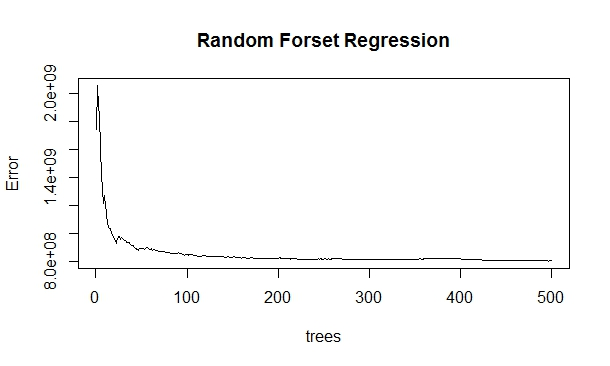
\includegraphics[width=\linewidth]{Figure4}
\caption{Error Rates For Random Forest}
\label{fig:Figure4}
\end{figure}

With this data in Kaggle we got a score of 0.29392. To improve our prediction we tried Ridge Regression and Lasso Regression Algorithm.

Before applying Lasso Regression we have done tuning of the parameters to get the best output. Ridge Regression or Lasso Regression varies mainly for the $\alpha$ . So, we tried to apply the best fit for $\alpha$.
After tuning $\alpha$ and plotting it, we got the following graph Figure~\ref{fig:Figure5}. 
\begin{figure}[ht]\centering % Using \begin{figure*} makes the figure take up the entire width of the page
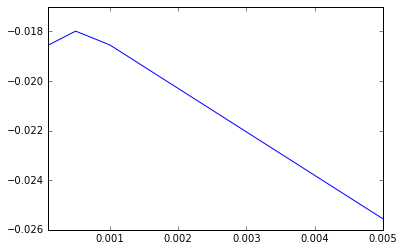
\includegraphics[width=\linewidth]{Figure5}
\caption{Tuning of $\alpha$ For Regression }
\label{fig:Figure5}
\end{figure}

After performing Lasso regression we have plotted the co-efficients (Figure~\ref{fig:Figure1}) to analyze the nature of the result.
As we can see the formation of co-efficients are giving us a proper linear relation around the regression line. So we considered this model to be the best fit for this data. 

\begin{figure}[ht]\centering % Using \begin{figure*} makes the figure take up the entire width of the page
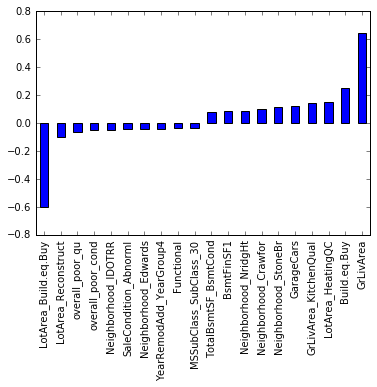
\includegraphics[width=\linewidth]{Figure1}
\caption{Coefficients in the Model}
\label{fig:Figure1}
\end{figure}

\subsubsection{Results}

After applying Lasso we got prediction variable shown in Figure~\ref{fig:Figure2}.
\begin{figure}[ht]\centering % Using \begin{figure*} makes the figure take up the entire width of the page
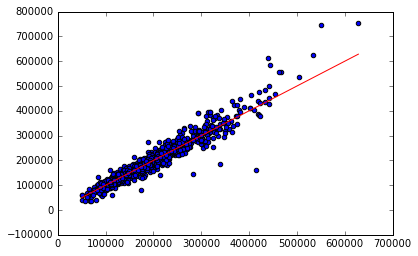
\includegraphics[width=\linewidth]{Figure2}
\caption{Regression Line}
\label{fig:Figure2}
\end{figure}

Applying Lasso we improved our score a lot and now our score is 0.12188.


\subsection{Outbrain Click Prediction} 

\subsubsection{Experiments with three features }\label{threefeatures}
In this experiments, we used three features, including topics, categories and campaign, to build a FFM model using 10\% of training data. The best validation logloss under different parameter settings are shown in table~\ref{tab:tuning0}. The best parameter settings is k = 20, lambda=0.0000005 and eta =0.05. This solution got LB score 0.61917.

\begin{table}[!htbp]
\begin{center}
 \begin{tabular}{ c|c|c|c|c|c }\hline\hline
k     &    lamba	  &   eta  & va\_logloss  &  iteration  &  tr\_logloss  \\ \hline\hline
4     &    0.00002   & 0.2    &   0.45918        &    20   &     0.45583 \\
10   &     0.00002  &  0.2    &   0.45831       &       7      &   0.45349 \\
15    &    0.00002   & 0.2    &   0.45811       &        5     &    0.45330\\
20    &    0.00002  &  0.2    &   0.45801       &        4    &     0.45380\\
25    &    0.00002   & 0.2   &    0.45808       &        4   &      0.45306\\
20    &    0.00005  &  0.2    &   0.45863      &        5   &      0.45373   \\   
20    &    0.00001  &  0.2  &     0.45781      &        4   &      0.45331   \\
20     &   0.000005 &  0.2  &     0.45772     &         4   &      0.45306    \\  
20      &  0.000002 &  0.2  &     0.45768     &         4   &      0.45291    \\  
20      &  0.000001 &  0.2  &     0.45766     &         4   &      0.45286      \\
20      &  0.0000005 & 0.2 &      0.45765     &          4  &       0.45283      \\
20     &   0.0000001&  0.2 &      0.45765     &          4  &       0.45281      \\
20    &    0.0000005 & 0.1  &     0.45717     &          9   &      0.45112   \\
20    &    0.0000005 & 0.05  &    0.45703(*) &         24  &       0.45071  \\
20   &     0.0000005 & 0.02   &   0.45719    &        100  &       0.45123    \\  
20    &    0.0000005 & 0.01 &     0.45896     &        100   &      0.45672   \\ \hline\hline
  \end{tabular}
\end{center}
\caption{Parameter tuning with three features}\label{tab:tuning0}
\end{table}

\subsubsection{Experiments on leakages}\label{leakageexperiments}
Based on the best solution from section~\ref{threefeatures}, we added leakage information. If the leakage exists for specific record of user clicking on the ads, then the score assigned to the pair of (display\_id, ad\_id) is 1.0 in spite of the original scores assigned by FFM. We experimented on three kinds of leakages, they are:
\begin{itemize}
\item leakAfter: the timestamps of the users visiting the documents are after the timestamp of associate display, because it's not possible that the users visits the documents before they clicks on the associated ads. 
\item leakIn10Mins: we consider that if the visiting behavior is too far way from the time that they click on the ads, the specific visiting behavior might not because the users clicks on that specific ad (i.e., it's from clicking on other ads).
\item leakWithTraffic1:  traffic\_source information in page\_views is provided. If traffic\_source is 1, it means the visiting activity comes from internal. This could be interpreted that users click on the ads to land on to the documents. 
\end{itemize}
\begin{table}[!htbp]
\begin{center}
 \begin{tabular}{ c|c|c }\hline\hline 
Leakage  & numOfRecords   &  LB scores \\ \hline \hline
None  &  & 0.61917 \\
leakAfter  &  270674 &  0.63612   \\
leakIn10Mins &  250297  &  0.63541  \\
leakWithTraffic1 & 270565   &  0.63612  \\ \hline \hline
\end{tabular}
\end{center}
\caption{Leakage tuning}\label{tab:leakagetuning}
\end{table}
From table~\ref{tab:leakagetuning}, it's obvious that the leak makes a big different for the prediction by improving the LB score 0.01695. However, these three leakages we are experimenting on have very similar outcomes. It's easy to understand as the number of records are very similar. What's interesting is that leakIn10 Mins got a little bit lower score. This also shows that there are a number of records for which users wait for a long time to click on the ads when they surf on the webpages, which is actually common in the real situation because people will firstly read the webpages they are looking for, or sometime people are interrupted while they are visiting webpages.

\subsubsection{Our best solution}
After performing many experiments, we found out that adding the feature campaign\_id based the solution from section~\ref{threefeatures} will help the prediction a lot. Table~\ref{tab:tuning} shows the best validation logloss lies on the parameter settings with k = 10, lambda=0.0000005 and eta = 0.05.

\begin{table}[!htbp]
\begin{center}
 \begin{tabular}{ c|c|c|c|c|c }\hline\hline 
k      &   lamba	 &    eta &   va\_logloss  &  iteration  &  tr\_logloss \\ \hline \hline
4     &    0.00002  &  0.2    & 0.44398     &           9    &  0.43276      \\
10    &    0.00002  &  0.2    & 0.44326      &          3   &   0.43822     \\
20    &    0.00002  &  0.2    & 0.44359        &        3    &  0.43679     \\
10    &    0.00005  &  0.2    & 0.44338        &        4    &  0.43603      \\
10    &    0.00001  &  0.2    & 0.44321     &           3    &  0.43793      \\
10    &    0.000005 &  0.2    & 0.44321      &          3   &   0.43778       \\ 
10    &    0.000001 &  0.2    & 0.44322        &        3    &  0.43764     \\
10    &    0.000005 &  0.1    & 0.44285          &      6    &  0.43544     \\
10    &    0.000005  & 0.05   & 0.44287   &             15  &   0.43426    \\
10    &    0.000005  & 0.02  &  0.44299    &            70   &  0.43285      \\
20    &    0.000005  & 0.1   &  0.44284      &          5    &  0.43455     \\
20    &    0.0000005 & 0.05  &  0.44269     &           11  &   0.43313    \\
30    &   0.0000005 & 0.05   & 0.44266  (*)   &            9 &     0.43340   \\  
40    &   0.0000005 & 0.05  &  0.44267        &        8     & 0.43348 \\ \hline\hline
  \end{tabular}
\end{center}
\caption{Parameter tuning}\label{tab:tuning}
\end{table}

From the section~\ref{leakageexperiments} we know that three kind of leakages get similar outcomes. By adding leakAfter to the best parameter settings in Table~\ref{tab:tuning}, we got our best solution with LB score 0.64077. By comparing table~\ref{tab:tuning} and table~\ref{tab:tuning0}, a clear validation logloss improvement is gained by adding the new features, which also indicates that proper features combination impacts more than parameter tuning as it provides different upper bound. The parameter tuning can only provide very limited improvements on the validation logloss.


\section{Summary and Conclusions}\label{conclusion}

This report provides a understanding of the two problems and our approaches to solve them. By experimenting on feature selections, feature engineering , models and also data leakages, we continued to improve our solution. From these two projects, we learned the following:
\begin{itemize}
\item Feature engineering is very important. For house prices project, we experimented on different models but got similar accuracies. However, by doing feature engineering in very fine-grained level, both the LB scores and ranks are improved a lot. 
\item Sampling and Streaming are useful for big data. We found out that by using only 10\% of training data, we can get very similar outcomes under large data settings. This helps us to solve large dataset in small machines, which is a great helpful guidance for any other data mining work. In addition, streaming is definitely helpful for dealing with large amount of data.
\item Data leakage impacts a lot. Data leakage is something we won't learn from the textbooks. It's something that sometimes hard, or even impossible to find. But it provides some kind of ground truth to some extent, which will improve the prediction a lot.
\item Features are more important than parameter tuning. We did a lot of parameter tuning, especially in Outbrain click prediction project. However, it's very clear from our experiments that the parameter tuning only helps in a very limited fashion. We interpret this as the proper feature combination provides the upper bound of the prediction  and the parameter tuning is used for reaching to that upper bound.
\end{itemize}


%------------------------------------------------
\phantomsection
\section*{Acknowledgments} % The \section*{} command stops section numbering
We would like to express special gratitude to our Data Mining Professor Mehmet Dalkilic to give us this special opportunity to be part of the Kaggle project.We are also thankful to the Assistant Instructors who helped us with any kind queries and support we asked for. Secondly we are grateful to Kaggle, using which we got lot of approaches to build our model, following that it gave us the opportunity to do researches with various model. Finally we are thankful to Indiana University Bloomington to offer  Data Mining course whose part of this project is, and Karst site to work with huge amount data . It opened a new door to handle data and do proper analysis on those data. This project consumed huge amount of work, research and dedication. These would not have been possible if we did not get support. Therefore, we would like to extend our sincere gratitude to all.

\addcontentsline{toc}{section}{Acknowledgments} % Adds this section to the table of contents
 
%----------------------------------------------------------------------------------------
%	REFERENCE LIST
%----------------------------------------------------------------------------------------
\phantomsection
\bibliographystyle{unsrt}
\bibliography{sample}

%----------------------------------------------------------------------------------------

\end{document}